\Section{Tile Implementation}
\label{sec:tile implementation}

  The macro system described in the previous section allows us to make any desired subset of a textual
language available for viewing in graphical form.  The textual code is
parsed to create a parse tree.  In this section, we describe the conversion to
graphical tiles from the parse tree, as well as conversion in the opposite direction.

\SubSection{Conversion To Graphical Tiles}
For each macro application, the parser creates an instance of the JavaScript
``class'' {\tt Tile} that represents a node in the parse tree.
There are different kinds of {\tt Tile} objects to represent different
types of syntax nodes; we provide pre-made {\tt Tiles} for each basic JavaScript construct such as {\tt
if}, {\tt while}, etc. so that these
can be also represented visually.  These different {\tt Tiles}
delegate to a ``superclass'' called {\tt GenericTile}, which
defines common behavior for all tiles; the specific tile types 
specialize this inherited behavior as appropriate.

  A method called {\tt makeTile()} is implemented by the {\tt Tile}s.
In the TileScript implementation, this method escapes to underlying
Smalltalk code that creates the graphical tile representation in the
Morphic GUI framework.  Since the tiles can be nested, {\tt
makeTile()} is also called recursively to create nested graphical
tiles.

\begin{figure}[tp]
\centering
\scalebox{0.4}{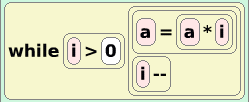
\includegraphics{hypowhile.eps}}
\caption{The appearance of {\tt while} statement with default look.}
\label{fig:hypo while}
\end{figure}

\begin{figure}[tp]
\centering
\scalebox{0.4}{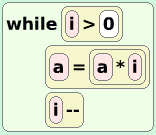
\includegraphics{realwhile.eps}}
\caption{The appearance of {\tt while} statement with customized look.}
\label{fig:real while}
\end{figure}

  We could have used a single, universal, graphical
representation for every macro, since all macros
have the same structure (i.e., one parent and zero or more children
nodes.)  Figure \ref{fig:hypo while} shows a hypothetical visual of the
{\tt while} statement in this generic way.  The generic tile would be
created with a list of sub-tiles, which would then be laid out in a simple
manner.

  However, we would like to provide better looking, better-suited, and more distinctive, tiles for the
most commonly used basic language constructs.  For example, the graphical
representation of {\tt while} actually looks like Figure \ref{fig:real
while}.  

  The specialized look of such a tile is created by hand in Morphic.
Morphic provides a direct manipulation interface for creating and
copying ``Morphs'' (``Morph'' is the basic graphic object in Morphic), for changing
their size, color, border, etc., and most notably for embedding them into
one another.  By using this interface, we manually create a Morph structure
that serves as the ``template'' for a particular tile.

  The tile designer may embed as many ``spacer'' Morphs, and other cosmetic Morphs, as he wishes, to lay
things out nicely and to create precisely the appearance he prefers.  He then needs to designate (via a menu) a morph to represent each ``hole'' to be
filled by tiles dropped by the user during drag-and-drop tile scripting; each  ``hole' Morph'' is subsequently marked with a distinctive Morphic  ``property'' so that the TileScript
system can know which morphs are to be replaced.  In the case of {\tt while}, for example, there are two holes' to be marked, one for the boolean expression to be evaluated, and another for the statement(s) to be repeatedly executed.

  In the implementation of {\tt makeTile()} for a tile which has such a user-defined
graphical tile template, the template is deeply copied and then
the Morphs that represent the holes are replaced by the tiles that represent
sub-trees.

  The end-user can easily use the same mechanism to create customized tiles to suit his personal taste.  For {\tt repeat}, for
example, the end-user would assemble Morphs and make a good-looking
Morph with (more than) two submorphs.  He would then identify two
morphs (the iteration count and the body) via the UI.  Once the user
is happy with the look, TileScript stores the Morph as the new
template for {\tt repeat}.

  Note that it is not strictly necessary to create a customized look for
a user-defined tile; the generic tile can provide the same editing
functionality.

  When a macro node in the parse tree contains a non-macro (i.e.,
textual) node, a special kind of tile that behaves as a text field is
instantiated.  The layout algorithm of these tiles (including the text
field tile) is simple at this point and resulting morphs tend to be
sparse when the user mixes textual code and tiles.

  Needless to say, the tile representation can be edited graphically.
The user may obtain new tiles from any of the available
templates, drag-and-drop them to construct a function, or delete
tiles by dragging them out of structure, and he can type in expressions in the text
fields.

  Each of the basic constructs in textual code (such as {\tt
while}, {\tt if}, or a function application), has its own pre-defined macro.

\SubSection{Conversion from Graphical Tiles}

  So far we have explained how to create a graphical representation from
textual code that contains macros.  To enable graphical
editing by the user, we also need a way to convert the
graphical representation back to a parse tree and to textual code.

  If we look at a graphical tile (represented as a Morph) in the
script, there are submorphs that are marked as particular sub-nodes in
a tree.  The converter recursively looks at the sub trees in the
Morph and converts them to parse trees.

  For a user-defined tile, the same macro definition can be used to do
the conversion from tiles to the macro node.  The macro specifies the
name of tile, and the names (and numbers) of arguments.  As long as
the user marks the morphs that represent the sub-trees (provided as
arguments) properly, the converter can visit the submorphs and convert
them to partial parse nodes.  Then, the parse node object for the user-defined tile itself
is created with these sub-trees.

  Each parse node knows how to convert itself to textual code, which makes it possible for
parse trees to be rendered as text.  In the current
implementation, the indentation and layout in the original text is
lost even if the user were only to write some textual code, convert it to the
tiles, and then go back to textual code without modifying the tiles; we are
planning to add more attributes to parse tree nodes so that
properties such as comments, indentation levels, and positions in the
original source code are preserved when possible.

\SubSection{Conversion from Base JavaScript to Macros}
  It is also useful to be able to convert arbitrary textual code written in the
base JavaScript language (i.e., without macros) to the form with macros.  To do
this, we provide a macro definition for every JavaScript construct.
The definition of {\tt @if} above is an example of such a macro.  By
running a visitor that converts JavaScript constructs to macros,
one can convert the textual JavaScript code to tiles.
